\section{System Architecture}

A general concern when designing large systems is the accidental
complexity\cite[p.~8-9]{holt2004uml} one may create by poor design choices early
on. Many solutions designed to reduce accidental complexity are based around
software systems, and sacrifices performance in both the time domain and in the
space domain\cite{moseley2006out}. While these solutions may be applicable
within hardware systems where these kinds of performance degradations are not a
problem, it is unacceptable in systems where one or multiple of the system
requirements are a performance increase in one or both of these domains. As one
of our main requirements is focus on performance, we have to accept a certain
level of inherent complexity.

\begin{figure}[h]
  \centering
  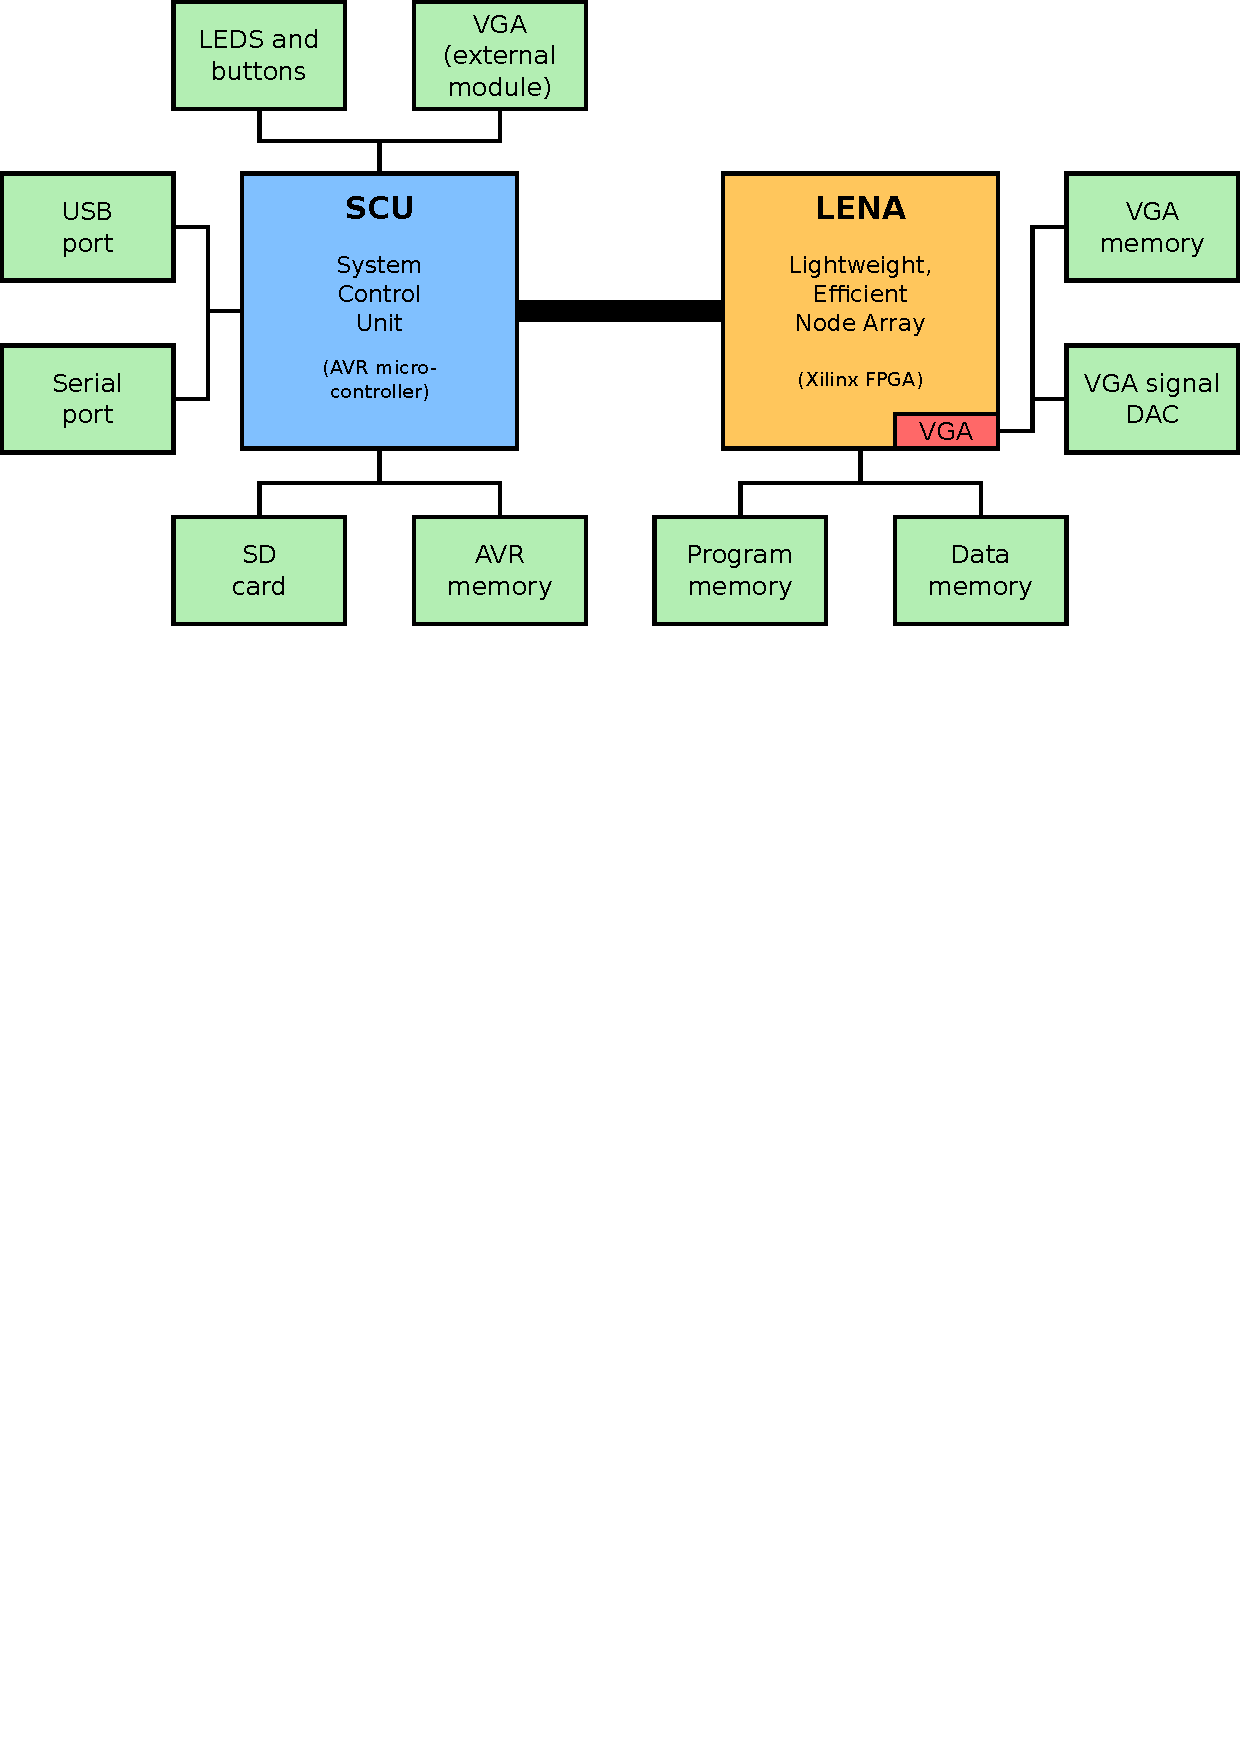
\includegraphics[width=\linewidth,clip,trim=0 18cm 0 0]
                  {fig/sys-over/arch-fig.pdf}
  \caption{System Architecture}
  \label{fig:sys-over-arch-fig}
\end{figure}


To remedy the complexity which comes from our requirements, we focused on making
it possible to isolate errors and make it possible to test the individual
components as fast as possible: The LENA architecture was tested through VHDL
test benches, the VGA component in the LENA architecture was tested with LEDs
and buttons on the board, and the AVR part of the LENA system was tested through
the VGA contact on the board. By doing this, we can safely assume that errors
occuring when connecting different components is due to errors in the protocol
implementation(s).

Figure \ref{fig:sys-over-arch-fig} shows our resulting architecture. Buttons and
LEDs made it easy to confirm that the VGA operates properly for simple
programs. A VGA connector made it possible to quickly test and debug the VGA
implementation on the LENA architecture. We also included a VGA connector
connected to the AVR, in case the LENA architecture would be unable to work the
VGA part.

To be able to process data, we need an I/O device which serves the machine with
data it should process. As we were unsure of what would be the easiest to
implement, we included both a serial, USB and SD card on the PCB.

The LENA architecture has three different memory components: One for the VGA
component, one for instructions and one for data. The main reason for this is
that an image processing system in general need much memory. The VGA module
needs to constantly send out the image to the VGA port, so it needs to keep the
old image in memory. The LENA architecture should have one image in memory which
it can send to the SIMD nodes, and one image which is currently read from the
SCU to memory. In addition, one would have to read data instructions as well. As
all these different parts require relatively much memory, and as they all are
frequently accessed, it would be favourable to have them in different parts to
be able to parallelise it.
